Today, we'll take our first look at interacting theories in detail! Let's first complete our description of the interaction picture. Operators in the interaction picture evolve in time by the free Hamiltonian:
%
$$O_I(t) \equiv e^{iH_0t}O_S e^{-iH_0t},$$
%
with $O_S$ the Schr\"odinger picture operator, while states evolve by
\begin{equation*}
    \ket{\psi(t)}_I=e^{iH_0t}\ket{\psi(t)}_S
        =e^{-iH_{int}t}\ket{\psi(0)}_S.
\end{equation*}
Note that the interacting Hamiltonian also has an interaction picture counterpart,
\begin{equation}
    H_I\equiv (H_{int})_I=e^{iH_0t} H_{int} e^{-iH_0t}.
\end{equation}
In the context of our quantum fields,
$$\phi_I(x)=e^{iH_0t}\phi(\vec x)e^{-iH_0t}$$
so that the interaction picture field $\phi_I$ obeys the Klein-Gordon equation
$$(\p^2+m^2)\phi_I=0,$$ with solution
$$\phi_I(x)=\int \frac{d^3p}{(2\pi)^3 \sqrt{2E_p}} (a_{\vec p} e^{-ip \cdot x}+ a_{\vec p}^\dagger e^{ip \cdot x}).$$
Here, note that we're taking the four-vector inner product $p\cdot x$ as in the Heisenberg picture, with $p^0=E_p$ and $x^0=t$. We also see that
$\phi_I(t=0,\vec x)= \phi_S(\vec x),$ so the fields at $t=0$ agree with the Schr\"odinger picture fields.

As before,
$$[a_{\vec p},a_{\vec p'}^\dagger]=(2\pi)^3 \delta^3(\vec p - \vec p'),$$ 
with other brackets vanishing. Note that the state $\ket{0}$ (satisfying $a_{\vec p}\ket{0}=0$) is the vacuum of the free theory, not the interacting theory. This means we will have to be a little careful when we compute the transition amplitudes between states, since they are measured relative to vacuum fluctuations, which will start bubbling as soon as we turn on interactions. 

As operators, interaction picture fields are related to the Heisenberg picture ones by
$$\phi_H(t,\vec x)=e^{iHt} e^{-iH_0t} \phi_I(x) e^{iH_0t} e^{-iHt},$$
where $e^{-iH_0t} \phi_I(x) e^{iH_0t}=\phi_S(\vec x).$ We can also regroup the operators here to write
$$\phi_H(t,\vec x) = U(t,0)^\dagger \phi_I(t,\vec x) U(t,0),$$
where 
\begin{equation}
    U(t,t_0)\equiv e^{iH_0t} e^{-iH(t-t_0)}e^{-iH_0t_0}%e^{iH_0(t-t_0)}e^{-iH(t-t_0)}
\end{equation} is a unitary time evolution operator. $U$ is defined such that%
    \footnote{We can verify this first property by a quick computation:
    \begin{align*}
        U(t_1,t_2)U(t_2,t_3)&=\left(e^{iH_0 t_1}e^{-iH(t_1-t_2)}e^{-iH_0 t_2}\right)
        \left(e^{iH_0 t_2}e^{-iH(t_2-t_3)}e^{-iH_0 t_3}\right)\\
        &=e^{iH_0 t_1}e^{-iH(t_1-t_2)}e^{-iH(t_2-t_3)}e^{-iH_0 t_3}\\
        &=e^{iH_0 t_1}e^{-iH(t_1-t_3)}e^{-iH_0 t_3} = U(t_1,t_3).
    \end{align*}
    Note that $H$ and $H_0$ are by no means guaranteed to commute, so we cannot na\"ively group them together in an exponent, i.e. $e^{iH_0t}e^{-iHt}\neq e^{i(H_0-H)t}$. Operator exponentials are different. In doing this calculation, we were only allowed to add the exponents when the operator in the exponent was the same in both terms.}
%
$$U(t_1,t_2)U(t_2,t_3)=U(t_1,t_3)$$
%
and $U(t,t)=1$. Equivalently, we see that%
    \footnote{If this isn't obvious, note that since $\ket{\psi(t)}_S=e^{-iHt}\ket{\psi(0)}_S$, it follows that interaction picture states evolve as
    \begin{equation*}
        \ket{\psi(t)}_I=e^{iH_0t}\ket{\psi(t)}_S=e^{iH_0t}e^{-iHt}\ket{\psi(0)}_S=U(t,0)\ket{\psi(0)}_S=U(t,0)\ket{\psi(0)}_I,
    \end{equation*}
    since the states agree independent of picture at $t=0$. Applying the property that $U(t_1,t_2)U(t_2,t_3)$, we see that $\ket{\psi(t)}_I=U(t,t')\ket{\psi(t')}_I$ for general $t,t'$. So $U$ really does have the function of being a time evolution operator on interaction picture states. }
%
$$\ket{\psi(t)}_I=U(t,t')\ket{\psi(t')}_I.$$ 
%
That is, $U$ evolves interaction picture states in time.

Now, actually computing $U$ in terms of operator exponentials would be a pain, especially since we might have multiple fields doing their thing (creating and destroying particles) at different points in time. Based on the properties of $U$ we have defined, can we find a more tractable expression for the time evolution operator? 

By differentiating our expression for $U$ with respect to time, we see that
\begin{align*}
    i\frac{dU(t,0)}{dt} &= 
        i\left[iH_0 e^{iH_0 t}e^{-iHt}+e^{iH_0t}(-iH) e^{-iHt}\right]\\
    &= e^{iH_0t} (H-H_0)e^{-iHt}\\
    &= e^{iH_0t} (H_{int})_S e^{-iH_0t} e^{iH_0t} e^{-iHt}\\
    &= H_I(t) U(t,0),
\end{align*}
which tells us that the operator $U$ obeys the equivalent of the Schr\"odinger equation.

If $(H_{int})_I=H_I$ were just a function, we could solve this by $U=\exp[-i \int_{t_0}^t H_I(t')dt'].$ However, because $H_i$ is an operator, life is not so simple, as we have ordering ambiguities. The issue becomes clear when we write out the first few terms in the exponential:
\begin{equation}
    \exp[-i \int_{t_0}^t H_I(t')dt']=1-i \int_{t_0}^t H_I(t')dt'+\frac{(-i)^2}{2!}\left(\int_{t_0}^t H_I(t')dt'\right)^2.
\end{equation}
If we take the time derivative, Leibniz tells us that this quadratic term becomes
\begin{equation}
    -\frac{1}{2}\int_{t_0}^t H_I(t')dt' H_I(t)-\frac{1}{2} H_I(t) \int_{t_0}^t H_I(t')dt'.
\end{equation}
But this first term is a problem since the $H_I(t)$ is on the wrong side of the integral and we can't commute it through because $[H_I(t'),H_I(t'')]\neq 0 \text{ for }t'\neq t''$.

However, our differential equation for $U$ tells us that a solution for $U(t,t_0)$ is given by%
    \footnote{Easy to check. By the fundamental theorem of calculus (what a throwback), $i\frac{d}{dt}\left[1+(-i)\int_{t_0}^t dt' H_I(t')U(t',t_0)\right] =H_I(t)U(t,t_0)$ and $U(t_0,t_0)=1+(-i)\int_{t_0}^{t_0} dt' H_I(t')U(t',t_0)=1$, so it satisfies the boundary conditions.
    }
$$U(t,t_0)=1+(-i)\int_{t_0}^t dt' H_I(t')U(t',t_0).$$
%
Therefore we can substitute this expression for $U(t,t_0)$ back into itself to get the infinite series
$$U(t,t_0)=1+(-i)\int_{t_0}^t dt' H_I(t')+(-i)^2 \int_{t_0}^t dt' \int_{t_0}^{t'} dt'' H_I(t')H_I(t'')+\ldots.$$
From the ranges of integration, it's clear that the $H_I$s are automatically time-ordered-- for instance, $H_I(t'')$ always takes place at $t''\leq t'$. Note that we could have rewritten this last term as
\begin{align*}
    \int_{t_0}^t dt' \int_{t_0}^{t'} dt'' H_I(t')H_I(t'') &=
        \int_{t_0}^t dt'' \int_{t_0}^{t''} dt' H_I(t'')H_I(t')\\
    &=\int_{t_0}^t dt' \int_{t'}^t dt'' H_I(t'')H_I(t'),
\end{align*}
where in the first line, the range of integration is $t'\leq t''$, while in the second it is $t'' \geq t'$. Note that this expression is time-ordered too, so $H_I(t'')H_I(t')=T[H_I(t')H_I(t'')]$ for these limits of integration. It follows that the quadratic term can be written
\begin{align*}
    (-i)^2\int_{t_0}^t dt' \int_{t_0}^{t'} dt'' H_I(t')H_I(t'') &=
        \frac{(-i)^2}{2}\left[\int_{t_0}^t dt' \int_{t_0}^{t'} dt'' T[H_I(t')H_I(t'')]
        +\int_{t_0}^t dt' \int_{t'}^t dt'' T[H_I(t')H_I(t'')]\right]\\
    &=\frac{(-i)^2}{2} \int_{t_0}^t dt' \int_{t_0}^t dt'' T[H_I(t') H_I(t'')].
\end{align*}%In general we can exploit symmetry to write the second term as
%$$\frac{(-i)^2}{2!}\int_{t_0}^t dt' \int_{t_0}^t dt'' T(H_I(t')H_I(t'')$$ (where we've picked up a $2$ as a symmetry factor), and 
We can play the same game for higher-order terms, and we'll get a symmetry factor of $n!$ to a term with $n$ copies of $H_I(t')$. With the same limits of integration on $dt',dt'',$ etc., these higher-order terms look a lot like the power series expansion of an exponential. This leads us to make the following definition.
\begin{defn}
Using time ordering, we find that $U$ can be written compactly as
$$U(t,t_0)=T \exp \left\{-i\int_{t_0}^t dt' H_I(t')\right\},$$
which we call \term{Dyson's formula.} (Note that $U(t,t_0)=T \exp \set{+i\int_{t_0}^t dt' L_I(t')}$, in terms of the Lagrangian.) This is a formal result, but we usually just expand to some finite order in terms of the coupling constants which live in the interacting Hamiltonian $H_I$.
\end{defn}
This is the last bit of machinery we need to start computing scattering amplitudes in quantum field theory!

\begin{defn}
The time evolution used in scattering theory is called the \term{$S$-matrix} (S for scattering). The $S$ matrix is defined to be
$$S=\lim_{t\to \infty,t_0\to -\infty}U(t,t_0).$$
\end{defn}
We will consider interactions where the final state $\ket{f}$ and the initial state $\ket{i}$ are well-separated from each other and are far away from the interaction. Therefore, the initial and final states $\ket{i},\ket{f}$ behave like free particles, i.e. they are eigenstates of $H_0$.\footnote{This is a heuristically useful description but a little slippery in the details. A  priori, there's no reason that eigenstates of the free Hamiltonian should be eigenstates of the interacting Hamiltonian. If you prefer, you can think of the scattering amplitude as the overlap (as measured by the inner product) between initial free particle states and final free particle states, with the possibility for some interaction in between. Even if we started with free particle eigenstates, our interaction is sure to evolve these states to some new ones, but we can look at the overlap between the time evolved versions of the free particle states $U(t,t_0)\ket{i}$ and the final free particle states we're interested in, $\bra{f}.$}

This should seem at least plausible: at late/early times, the particles are well-separated and don't feel the effect of each other. As they approach, they may interact before going their separate ways. The scattering amplitude is then
$$\lim_{t\to\infty, t_0\to -\infty}\bra{f}U(t,t_0)\ket{i}=\bra{f}S \ket{i}.$$

Note that there are some cases that need to be treated differently, like bound states. For instance, a proton and an electron at low energies could interact to form a hydrogen atom, $p+e^-\to$ the bound state $(H)$. Here, the assumption that the particles end up well-separated is violated. It turns out that such solutions appear as poles in the $S$-matrix, but this is a more advanced topic and we won't discuss it further here.

Let's return to scalar Yukawa theory. Now, we'll drop the $I$ subscripts and assume uniformly that we are in the interaction picture. Discarding the kinetic and mass terms from the free theory, we are left with the interaction Hamiltonian
$$\cH = g \psi^* \psi \phi,$$
where $\psi$ and $\psi^*$ are (anti-)nucleons (e.g. a proton or neutron), and $\phi$ is a meson. What do each of these fields do?
\begin{itemize}
    \item $\phi$ has $a$ and $a^\dagger$ terms which destroy and create mesons, respectively.
    \item $\psi$ has $b$ and $c^\dagger$ terms, where $b$ destroys a nucleon and $c^\dagger$ creates an anti-nucleon.
    \item $\psi^*$ has $b^\dagger$ and $c$ terms, where $b^\dagger$ creates a nucleon and $c$ destroys an anti-nucleon.
\end{itemize}
Looking at the possible terms in the Hamiltonian, we can already see interesting behavior-- we'll have terms where nucleon-anti-nucleon pairs are created and destroyed, e.g. $b^\dagger c^\dagger a$ which destroys a meson and produces a nucleon-anti-nucleon pair. This contributes to meson decay, $\phi\to \psi\bar \psi$.%
    \footnote{When we talk about the fields, we use $*$, but when we denote antiparticles, we usually use the bar notation, e.g. an anti-$\psi$ is a $\bar \psi$.} 
What we recover is the leading order in $g$ term in the $S$-matrix, and an interaction that schematically looks like Fig. \ref{fig:mesondecay1}.

\begin{figure}
    \centering
    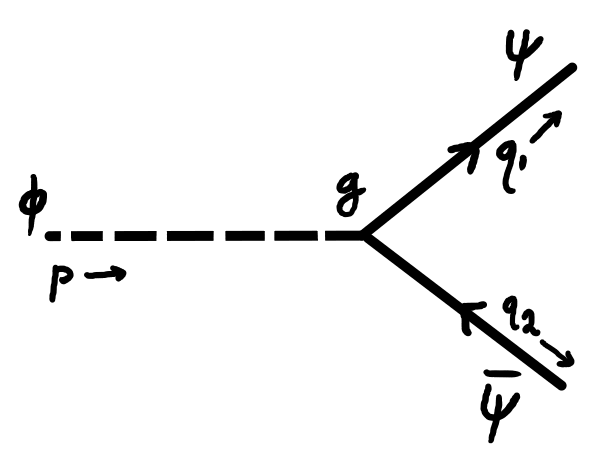
\includegraphics[width=0.5\textwidth]{2018/10/20181020_mesondecay.png}
    \caption{The Feynman diagram for meson decay, $\phi\to \psi\bar \psi$. Thinking perturbatively, this is the leading order behavior in the expansion of $\bra{f}S\ket{i}$ where $\ket{i}\sim a^\dagger \ket{0}$, the one-meson state, and $\ket{f}\sim b^\dagger c^\dagger \ket{0}$, the state with a nucleon and an anti-nucleon.}
    \label{fig:mesondecay1}
\end{figure}

At second order, $S$ can include more complicated terms like
$$g^2(b^\dagger c^\dagger a)(a^\dagger c b),$$
which describes nucleon-anti-nucleon scattering. We can draw a nice diagram for this process too, seen in Fig. \ref{fig:nucleonscattering1}.

\begin{figure}
    \centering
    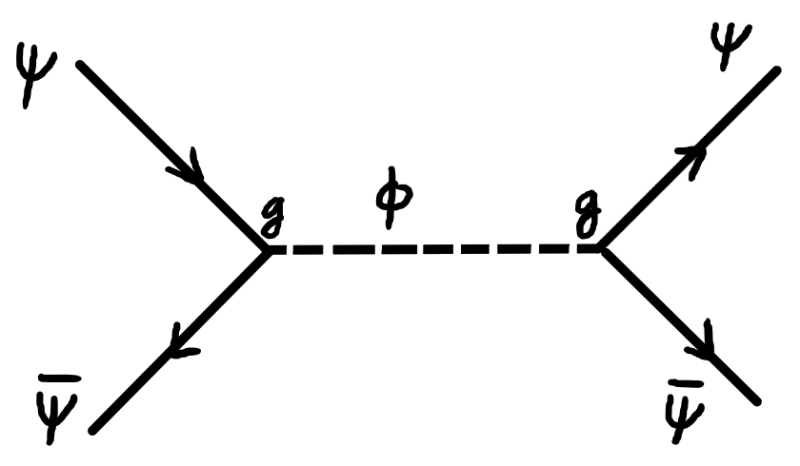
\includegraphics[width=0.5\textwidth]{2018/10/20181020_nucleonscattering.png}
    \caption{One Feynman diagram for nucleon-anti-nucleon scattering. Schematically, a nucleon and an anti-nucleon collide and annihilate into a meson, which then decays back to a nucleon and anti-nucleon. This isn't the only diagram at this order-- we'll see that there's also a contributing diagram where the nucleon and anti-nucleon exchange a meson and then go on their way.}
    \label{fig:nucleonscattering1}
\end{figure}

Returning to the case of meson decay, we have some $\phi$ meson going in with some defined momentum $\vec p$ as our initial state, and similarly we have $\psi,\bar \psi$ going out with some momenta $\vec q_1,\vec q_2.$ We can write these states as
$$\ket{i}=\sqrt{2E_p}a_{\vec p}^\dagger \ket{0}$$
and
$$\ket{f}=\sqrt{4E_{q_1}E_{q_2}}b_{\vec q_1}^\dagger c_{\vec q_2}^\dagger \ket{0}.$$
To zeroth order there is no interaction and the scattering amplitude is zero, so to leading order, we have
$$\bra{f}S\ket{i}=-ig \bra{f}\int d^4 x \psi^* (x) \psi(x) \phi(x) \ket{i} + O(g^2).$$
We'll compute this exactly next time and argue that the $O(g^2)$ corrections to this process are relatively small, arriving at our first quantum field theory scattering amplitude.